\documentclass[border=3mm,
               tikz,
               preview,
               qconvert
               ]{standalone}
\usepackage{pgfplots}

\begin{document}

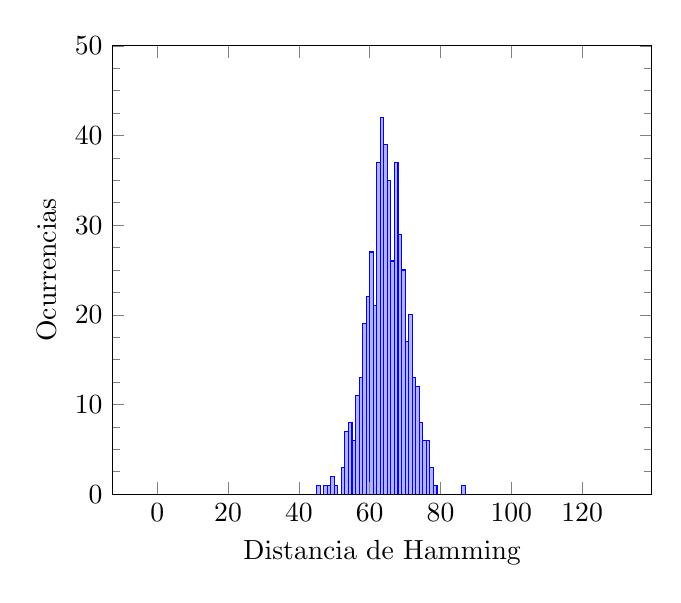
\begin{tikzpicture}
\begin{axis}[
    ymin=0, ymax=50,
    minor y tick num = 3,
    area style,
    ylabel = {Ocurrencias},
    xlabel = {Distancia de Hamming},
    ]
    \addplot+[ybar interval,mark=no] plot coordinates {

      (0, 0)
      (1, 0)
      (2, 0)
      (3, 0)
      (4, 0)
      (5, 0)
      (6, 0)
      (7, 0)
      (8, 0)
      (9, 0)
      (10, 0)
      (11, 0)
      (12, 0)
      (13, 0)
      (14, 0)
      (15, 0)
      (16, 0)
      (17, 0)
      (18, 0)
      (19, 0)
      (20, 0)
      (21, 0)
      (22, 0)
      (23, 0)
      (24, 0)
      (25, 0)
      (26, 0)
      (27, 0)
      (28, 0)
      (29, 0)
      (30, 0)
      (31, 0)
      (32, 0)
      (33, 0)
      (34, 0)
      (35, 0)
      (36, 0)
      (37, 0)
      (38, 0)
      (39, 0)
      (40, 0)
      (41, 0)
      (42, 0)
      (43, 0)
      (44, 0)
      (45, 1)
      (46, 0)
      (47, 1)
      (48, 1)
      (49, 2)
      (50, 1)
      (51, 0)
      (52, 3)
      (53, 7)
      (54, 8)
      (55, 6)
      (56, 11)
      (57, 13)
      (58, 19)
      (59, 22)
      (60, 27)
      (61, 21)
      (62, 37)
      (63, 42)
      (64, 39)
      (65, 35)
      (66, 26)
      (67, 37)
      (68, 29)
      (69, 25)
      (70, 17)
      (71, 20)
      (72, 13)
      (73, 12)
      (74, 8)
      (75, 6)
      (76, 6)
      (77, 3)
      (78, 1)
      (79, 0)
      (80, 0)
      (81, 0)
      (82, 0)
      (83, 0)
      (84, 0)
      (85, 0)
      (86, 1)
      (87, 0)
      (88, 0)
      (89, 0)
      (90, 0)
      (91, 0)
      (92, 0)
      (93, 0)
      (94, 0)
      (95, 0)
      (96, 0)
      (97, 0)
      (98, 0)
      (99, 0)
      (100, 0)
      (101, 0)
      (102, 0)
      (103, 0)
      (104, 0)
      (105, 0)
      (106, 0)
      (107, 0)
      (108, 0)
      (109, 0)
      (110, 0)
      (111, 0)
      (112, 0)
      (113, 0)
      (114, 0)
      (115, 0)
      (116, 0)
      (117, 0)
      (118, 0)
      (119, 0)
      (120, 0)
      (121, 0)
      (122, 0)
      (123, 0)
      (124, 0)
      (125, 0)
      (126, 0)
      (127, 0)


      
};
\end{axis}
\end{tikzpicture}
    \end{document}

